\chapter{Sensitivities for SBC-ININ-LAr Experiment}\label{cap:analisis}
\label{chap:sensitivity_sin2thetaW_NCR}

\section{Introduction}
This chapter presents the projected statistical sensitivity of a coherent elastic neutrino-nucleus scattering (CE$\nu$NS) experiment based on LAr target exposed to reactor antineutrinos, to two Standard Model parameters: the weak mixing angle $\sin^2\theta_W$ and the electron neutrino charge radius (NCR) $\langle r_{\nu_e}^2\rangle$. The results below correspond to different detector masses (10, 20, 100 and 200 kg), exposure times (100 and 200 days), and to the two limiting treatments of the QF discussed in the methodology chapter: an idealized QF $=1$ case and the realistic case computed from the Lindhard model for argon. The chapter reproduces the projected event rates, the $1\sigma$ confidence intervals extracted from the $\Delta\chi^2$ statistic, and the corresponding $\Delta\chi^2$ curves for each configuration.

\section{Calculation Parameters}
The results quoted throughout this chapter use the fixed inputs:
\begin{itemize}
\item $P = 1$ MW 
\item $d = 3$ m 
\item $t = 100$ or $200$ days 
\item $M_{\text{Detector}} = 20$, $100$ or $200$ kg 
\item $N_{\text{targets}} = 3\times10^{26}$ 
\item $1.5\times10^{27}$ or $3\times10^{27}$ 
\item $M = 39.95$ u $= 37.21$ GeV for the $^{40}$Ar nucleus 
\item $M_W = 80.379$ GeV, $G_F = 1.16\times10^{-11}\ \text{MeV}^{-2}$ 
\item $g_n^V = -\tfrac{1}{2}$ 
\end{itemize}
together with the Standard Model reference values $\left(\sin^2\theta_W\right)_{\text{SM}} = 0.22337$ and $\langle r_{\nu_e}^2\rangle_{\text{SM}} = -0.826\times10^{-32}\ \text{cm}^2$. The differential event rate follows the usual CE$\nu$NS convolution of the Huber-Mueller reactor flux with the CE$\nu$NS cross section, integrated over the recoil-energy window set by the ionization threshold $E_{I}^{\text{threshold}} \sim 100\ \text{eV}_{\text{ee}}$, which through the Lindhard quenching relation corresponds to $E_{R}^{\text{threshold}} \sim 400\ \text{eV}_{\text{nr}}$.

\section{Projected Event Rates}
Table~\ref{tab:event_rates} lists the expected number of events per day for each detector mass, separately for the two parametrizations of $g_p^V$ (pure $\sin^2\theta_W$ dependence, and the combined $\sin^2\theta_W$-NCR dependence), and for the two QF treatments.

\begin{table}[H]
\centering
\caption{Projected CE$\nu$NS event rates (events/day) as a function of detector mass, for $QF=1$ and for the Lindhard quenching model.}
\label{tab:event_rates}
\begin{tabular}{lcccc}
\hline
$g_p^V$ ($QF=1$) & 10 kg & 20 kg & 100 kg & 200 kg \\
\hline
$\propto \sin^2\theta_W$ & $\sim 10.1$ & $\sim 20.2$ & $\sim 101$ & $\sim 202$ \\
$\propto \sin^2\theta_W\left(1+\tfrac{1}{3}M_W^2\langle r_{\nu_e}^2\rangle\right)$ & $\sim 10.5$ & $\sim 21.1$ & $\sim 105$ & $\sim 211$ \\
\hline
\hline
$g_p^V$ (Lindhard QF) & 10 kg & 20 kg & 100 kg & 200 kg \\
\hline
$\propto \sin^2\theta_W$ & $\sim 2.2$ & $\sim 4.5$ & $\sim 22$ & $\sim 44$ \\
$\propto \sin^2\theta_W\left(1+\tfrac{1}{3}M_W^2\langle r_{\nu_e}^2\rangle\right)$ & $\sim 2.3$ & $\sim 4.7$ & $\sim 23$ & $\sim 46$ \\
\hline
\end{tabular}
\end{table}

The reduction of roughly a factor of $4$-$5$ in the expected rate between the $QF=1$ and Lindhard cases reflects the fraction of recoil events lost below the ionization threshold once the realistic quenching relation is applied, and it propagates directly into the widths of the confidence intervals discussed below.

\section{Results}
All intervals below are quoted at $68.27\%$ confidence level ($1\sigma$), obtained from the $\Delta\chi^2$ statistic defined in the methodology chapter, without including systematic correlations between $\sin^2\theta_W$ and $\langle r_{\nu_e}^2\rangle$.

\subsection{Without QF Influence}

\subsubsection{Sensitivity to \texorpdfstring{$\sin^2\theta_W$}{sin2thetaW}}
For an experiment with 100-day exposure and $QF=1$, the values at $1\sigma$ confidence level are given by:
\begin{itemize}
\item $\sin^2\theta_W = 0.223\pm0.007$, 10 kg detector.
\item $\sin^2\theta_W = 0.223\pm0.005$, 20 kg detector.
\item $\sin^2\theta_W = 0.223\pm0.003$, 100 kg detector.
\item $\sin^2\theta_W = 0.223\pm0.001$, 200 kg detector.
\end{itemize}

% \begin{figure}[H]
% \centering
% 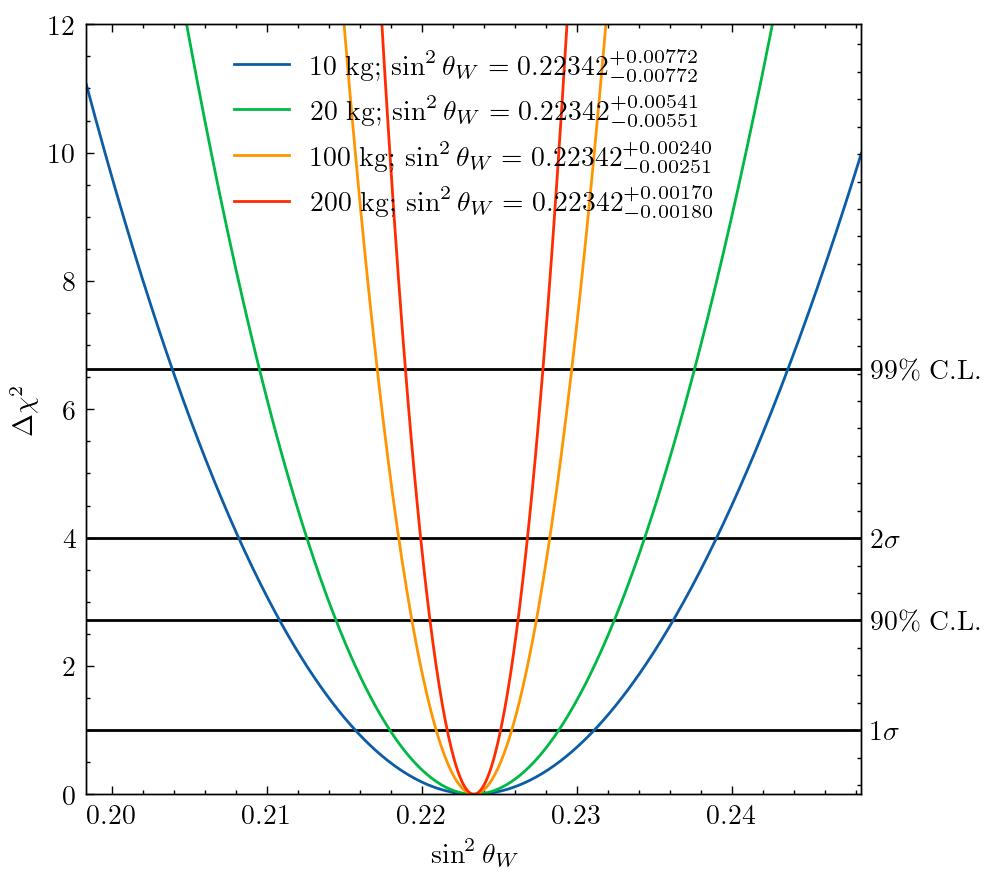
\includegraphics[width=0.5\textwidth]{figures/Figure_sin_100_NO_QF.png}
% \caption{$\Delta\chi^2$ curves for the parameter $\sin^2\theta_W$, experimental arrangement with 100-day exposure.}
% \label{fig:chi2_sin2thetaW_100d}
% \end{figure}

For an experiment with 200-day exposure and $QF=1$, the values at $1\sigma$ confidence level are given by:
\begin{itemize}
\item $\sin^2\theta_W = 0.223\pm0.005$, 10 kg detector.
\item $\sin^2\theta_W = 0.223\pm0.003$, 20 kg detector.
\item $\sin^2\theta_W = 0.223\pm0.002$, 100 kg detector.
\item $\sin^2\theta_W = 0.223\pm0.001$, 200 kg detector.
\end{itemize}

% \begin{figure}[H]
% \centering
% 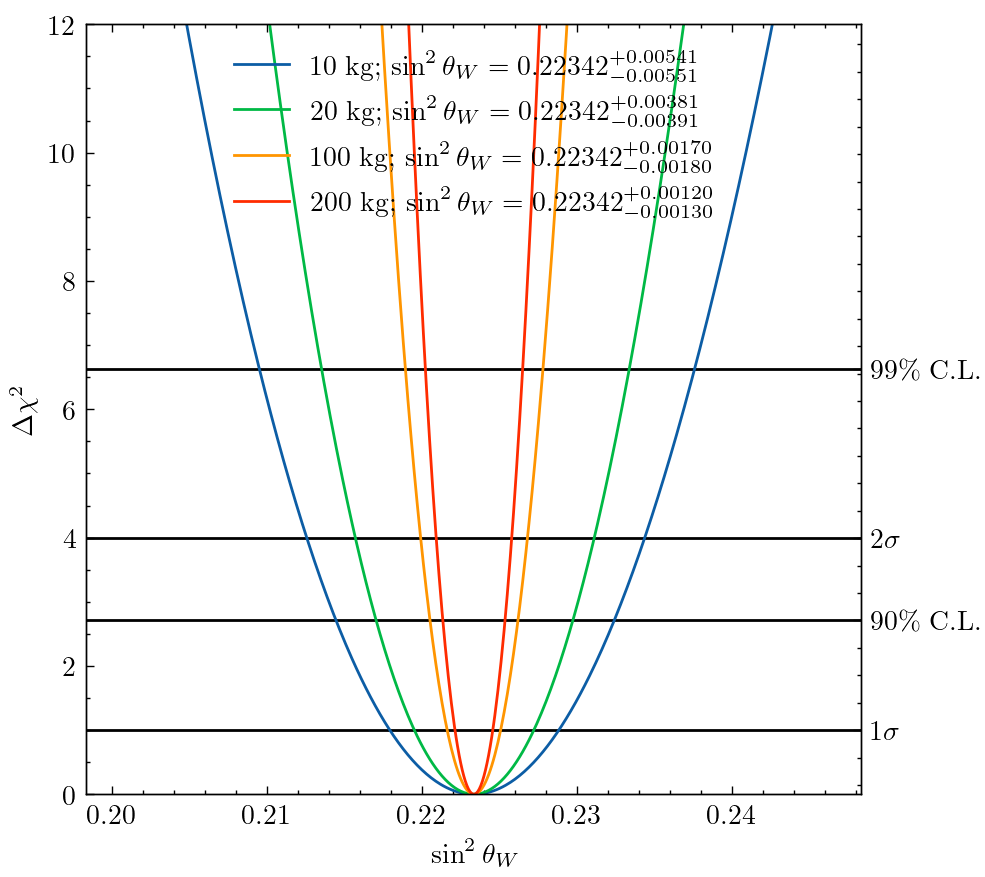
\includegraphics[width=0.5\textwidth]{figures/Figure_sin_200_NO_QF.png}
% \caption{$\Delta\chi^2$ curves for the parameter $\sin^2\theta_W$, experimental arrangement with 200-day exposure.}
% \label{fig:chi2_sin2thetaW_200d}
% \end{figure}

\begin{figure}[H]
\centering
\subfigure[100-day exposure.]{
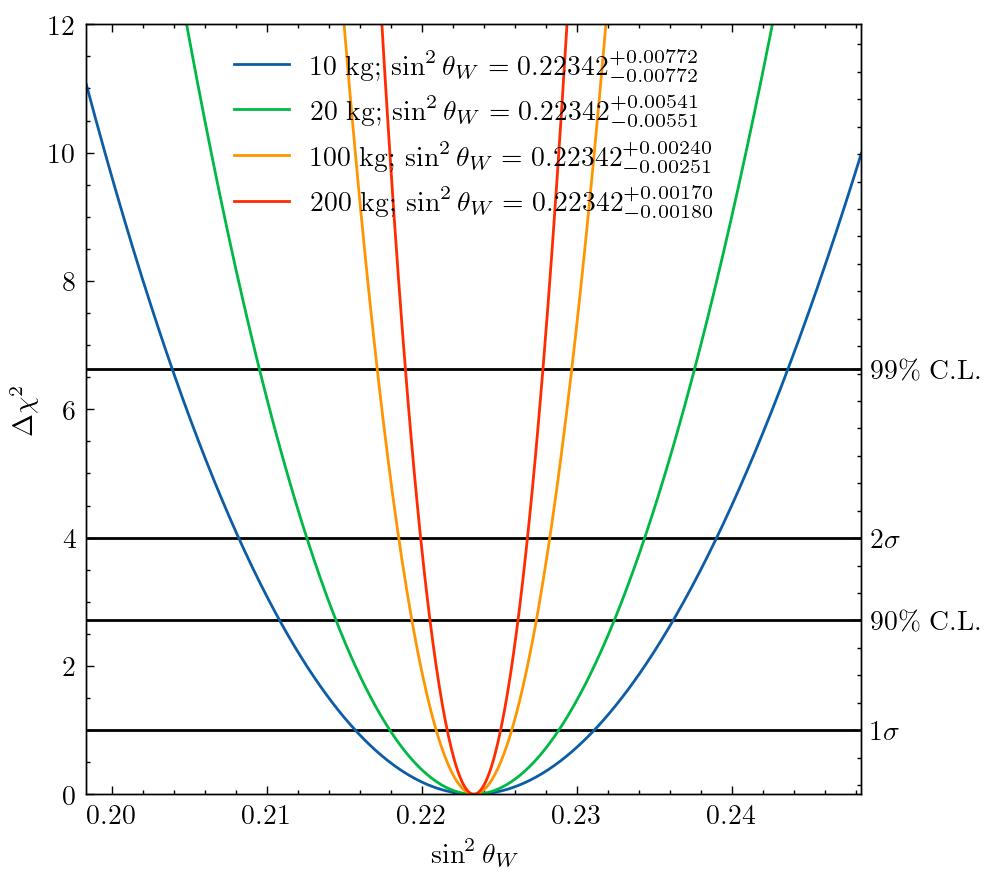
\includegraphics[width=0.48\textwidth]{figures/Figure_sin_100_NO_QF.png}
\label{fig:chi2_sin2thetaW_100d}}
\subfigure[200-day exposure.]{
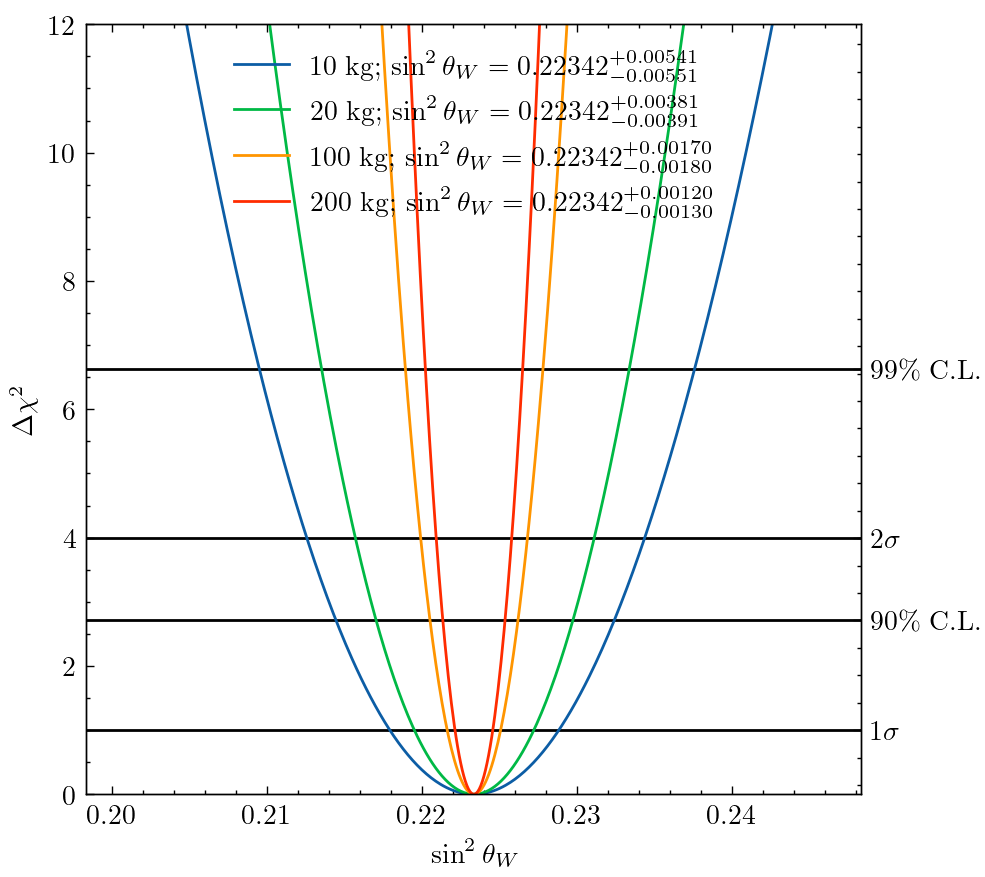
\includegraphics[width=0.48\textwidth]{figures/Figure_sin_200_NO_QF.png}
\label{fig:chi2_sin2thetaW_200d}}
\caption{$\Delta\chi^2$ curves for the parameter $\sin^2\theta_W$, without QF influence.}
\label{fig:chi2_sin2thetaW_noQF}
\end{figure}


\subsubsection{Sensitivity to \texorpdfstring{$\langle r_{\nu_e}^2\rangle$}{NCR}}
For an experiment with 100-day exposure and $QF=1$, the values at $1\sigma$ confidence level are given by:
\begin{itemize}
\item $\langle r_{\nu_e}^2\rangle = -8\pm6\times10^{-33}\ \text{cm}^2$, 10 kg detector.
\item $\langle r_{\nu_e}^2\rangle = -8\pm4\times10^{-33}\ \text{cm}^2$, 20 kg detector.
\item $\langle r_{\nu_e}^2\rangle = -8\pm2\times10^{-33}\ \text{cm}^2$, 100 kg detector.
\item $\langle r_{\nu_e}^2\rangle = -8\pm1\times10^{-33}\ \text{cm}^2$, 200 kg detector.
\end{itemize}

% \begin{figure}[H]
% \centering
% 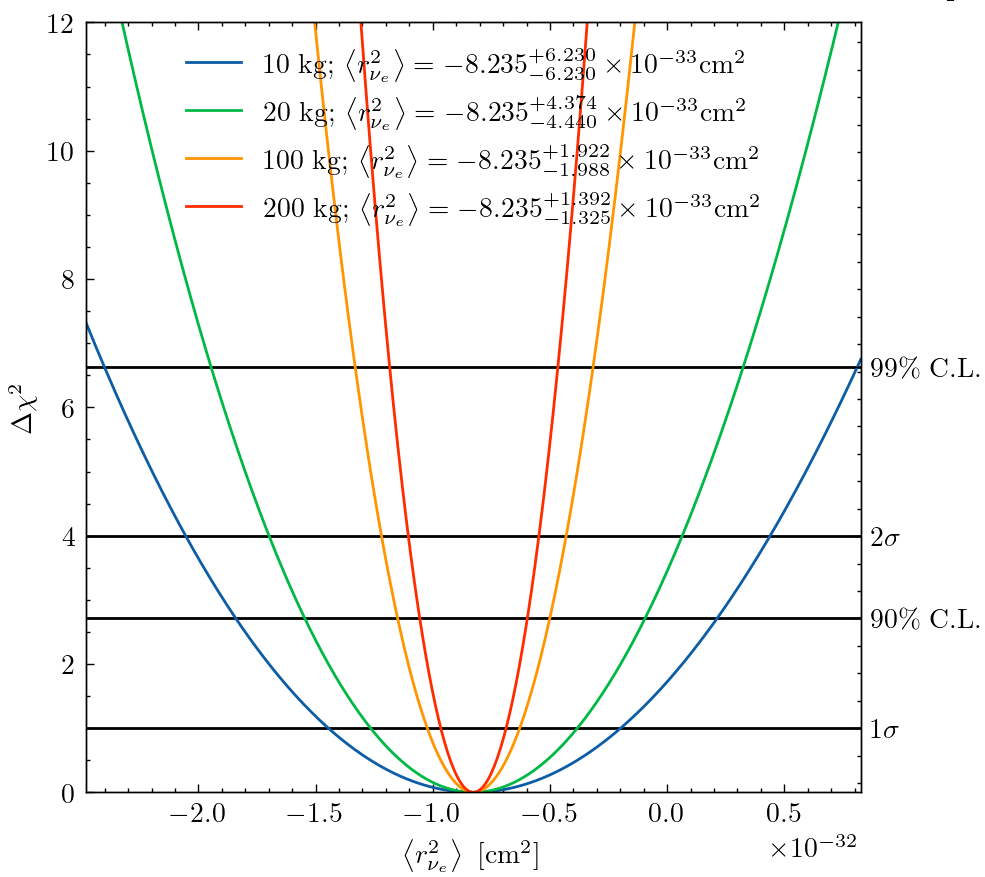
\includegraphics[width=0.5\textwidth]{figures/Figure_phi_100_NO_QF.png}
% \caption{$\Delta\chi^2$ curves for the parameter $\langle r_{\nu_e}^2\rangle$, experimental arrangement with 100-day exposure.}
% \label{fig:chi2_NCR_100d}
% \end{figure}

or an experiment with 200-day exposure and $QF=1$, the values at $1\sigma$ confidence level are given by:
\begin{itemize}
\item $\langle r_{\nu_e}^2\rangle = -8\pm4\times10^{-33}\ \text{cm}^2$, 10 kg detector.
\item $\langle r_{\nu_e}^2\rangle = -8\pm3\times10^{-33}\ \text{cm}^2$, 20 kg detector.
\item $\langle r_{\nu_e}^2\rangle = -8\pm1\times10^{-33}\ \text{cm}^2$, 100 kg detector.
\item $\langle r_{\nu_e}^2\rangle = -8.2\pm0.9\times10^{-33}\ \text{cm}^2$, 200 kg detector.
\end{itemize}

\begin{figure}[H]
\centering
\subfigure[100-day exposure.]{
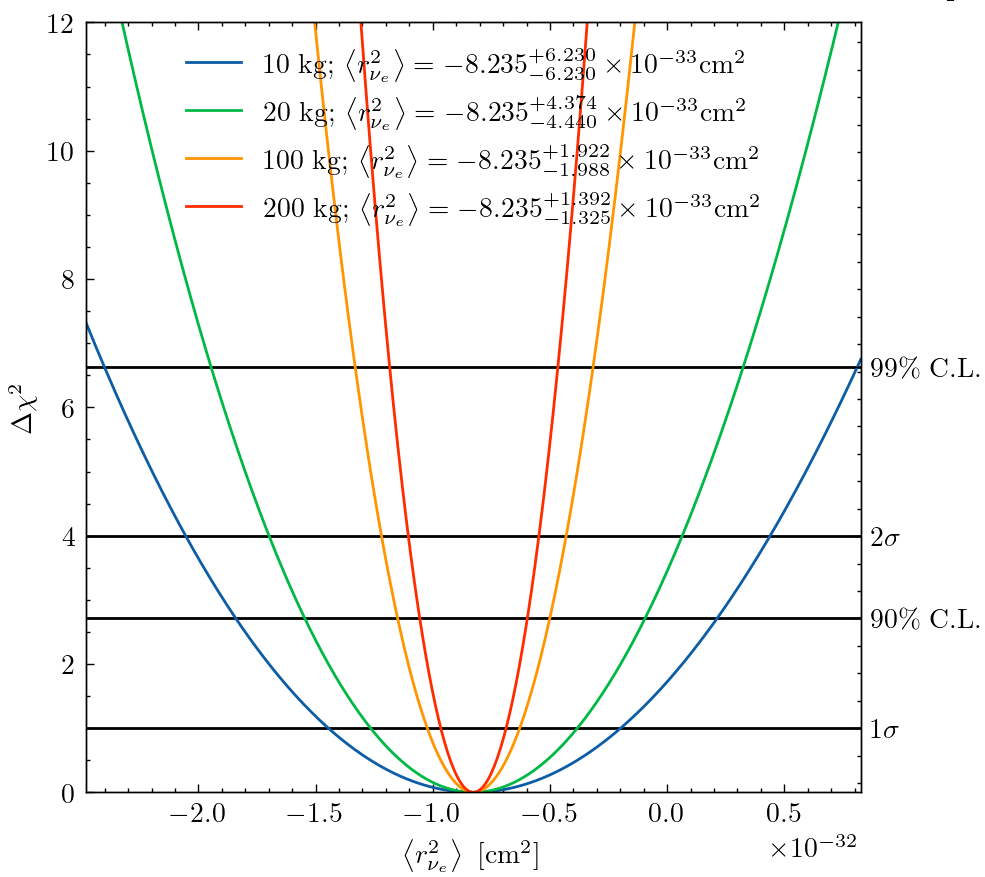
\includegraphics[width=0.48\textwidth]{figures/Figure_phi_100_NO_QF.png}
\label{fig:chi2_sin2thetaW_100d}}
\subfigure[200-day exposure.]{
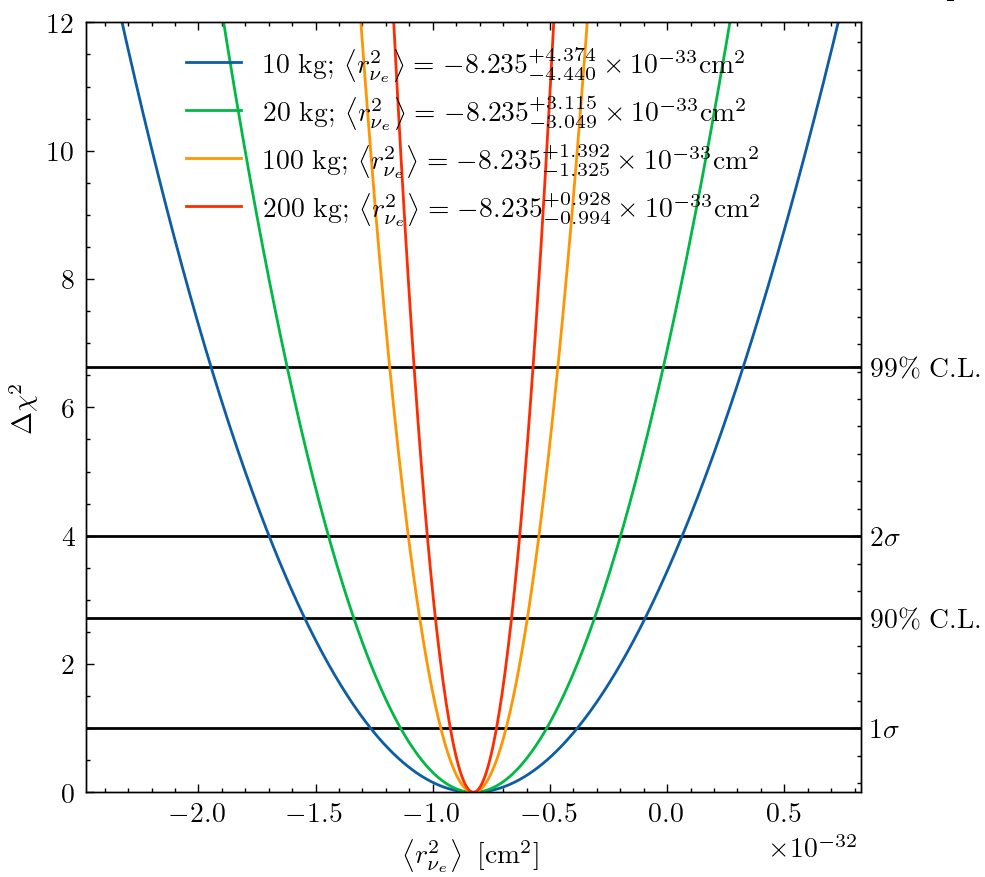
\includegraphics[width=0.48\textwidth]{figures/Figure_phi_200_NO_QF.png}
\label{fig:chi2_sin2thetaW_200d}}
\caption{$\Delta\chi^2$ curves for the parameter $\langle r^2_{\nu_e} \rangle$, without QF influence.}
\label{fig:chi2_sin2thetaW_noQF}
\end{figure}

\subsection{With QF Influence}

\subsubsection{Sensitivity to \texorpdfstring{$\sin^2\theta_W$}{sin2thetaW}}
Including the Lindhard quenching factor, the 100-day exposure yields 

$\sin^2\theta_W = 0.22\pm0.02$, 10 kg detector. 
$\sin^2\theta_W = 0.22\pm0.01$, 20 kg detector.
$\sin^2\theta_W = 0.223\pm0.005$, 100 kg detector. 
$\sin^2\theta_W = 0.223\pm0.003$, 200 kg detector.

% \begin{figure}[H]
% \centering
% 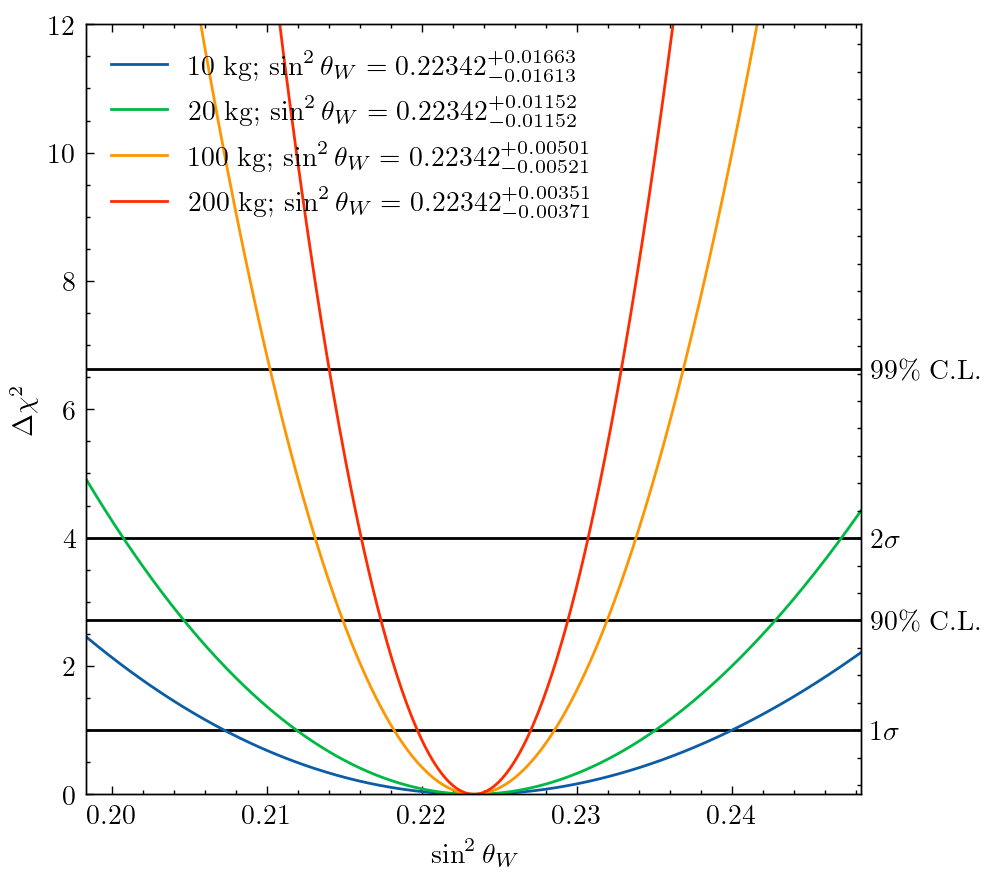
\includegraphics[width=0.5\textwidth]{figures/Figure_sin_100.png}
% \caption{$\Delta\chi^2$ curves for the parameter $\sin^2\theta_W$, experimental arrangement with 100-day exposure, including quenching factor.}
% \label{fig:chi2_sin2thetaW_100d_QF}
% \end{figure}

For an experiment with 200-day exposure, including the Lindhard quenching factor, the values at $1\sigma$ confidence level are given by:
\begin{itemize}
\item $\sin^2\theta_W = 0.22\pm0.01$, 10 kg detector.
\item $\sin^2\theta_W = 0.223\pm0.008$, 20 kg detector.
\item $\sin^2\theta_W = 0.223\pm0.003$, 100 kg detector.
\item $\sin^2\theta_W = 0.223\pm0.002$, 200 kg detector.
\end{itemize}

\begin{figure}[H]
\centering
\subfigure[100-day exposure.]{
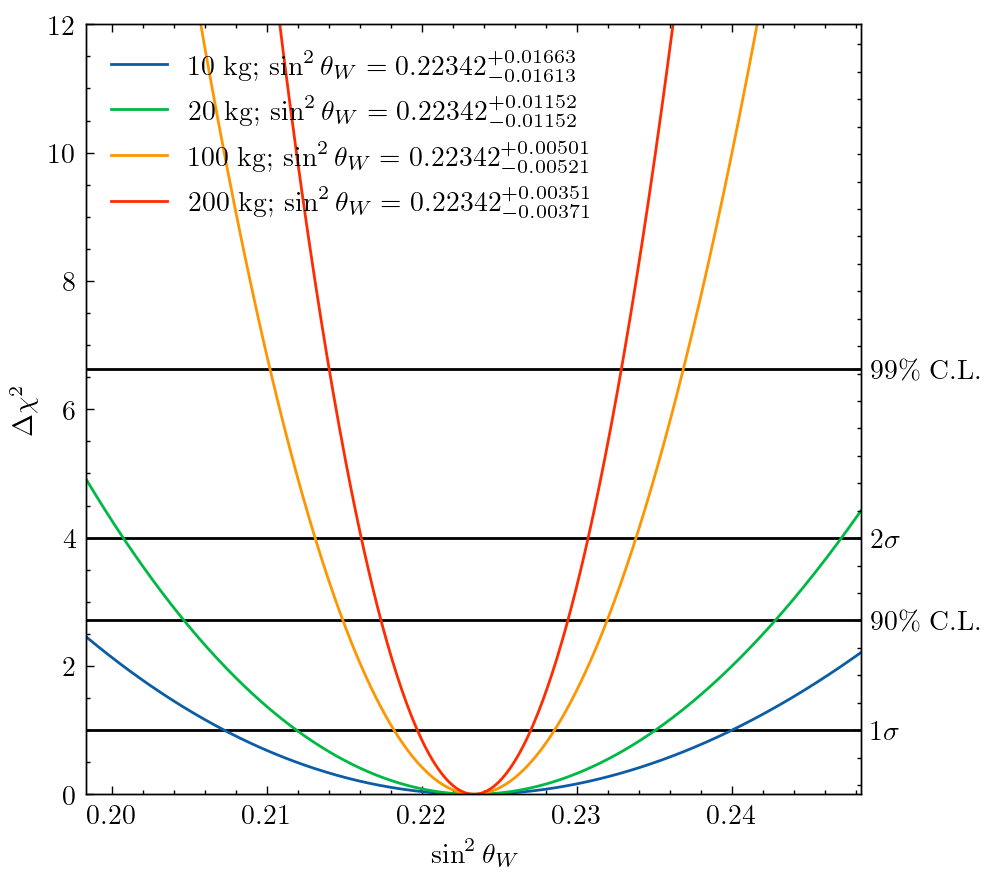
\includegraphics[width=0.48\textwidth]{figures/Figure_sin_100.png}
\label{fig:chi2_sin2thetaW_100d}}
\subfigure[200-day exposure.]{
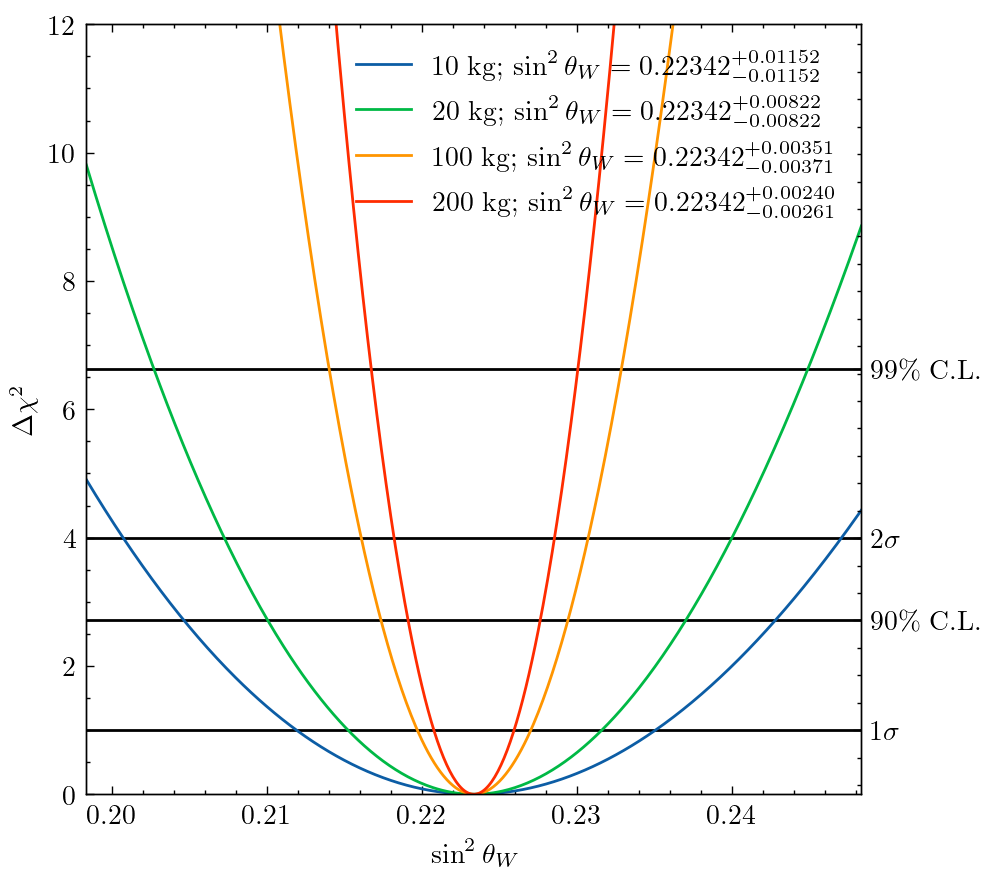
\includegraphics[width=0.48\textwidth]{figures/Figure_sin_200.png}
\label{fig:chi2_sin2thetaW_200d}}
\caption{$\Delta\chi^2$ curves for the parameter $\sin^2 \theta_W$, with Lindhard QF influence.}
\label{fig:chi2_sin2thetaW_noQF}
\end{figure}

% \begin{figure}[H]
% \centering
% 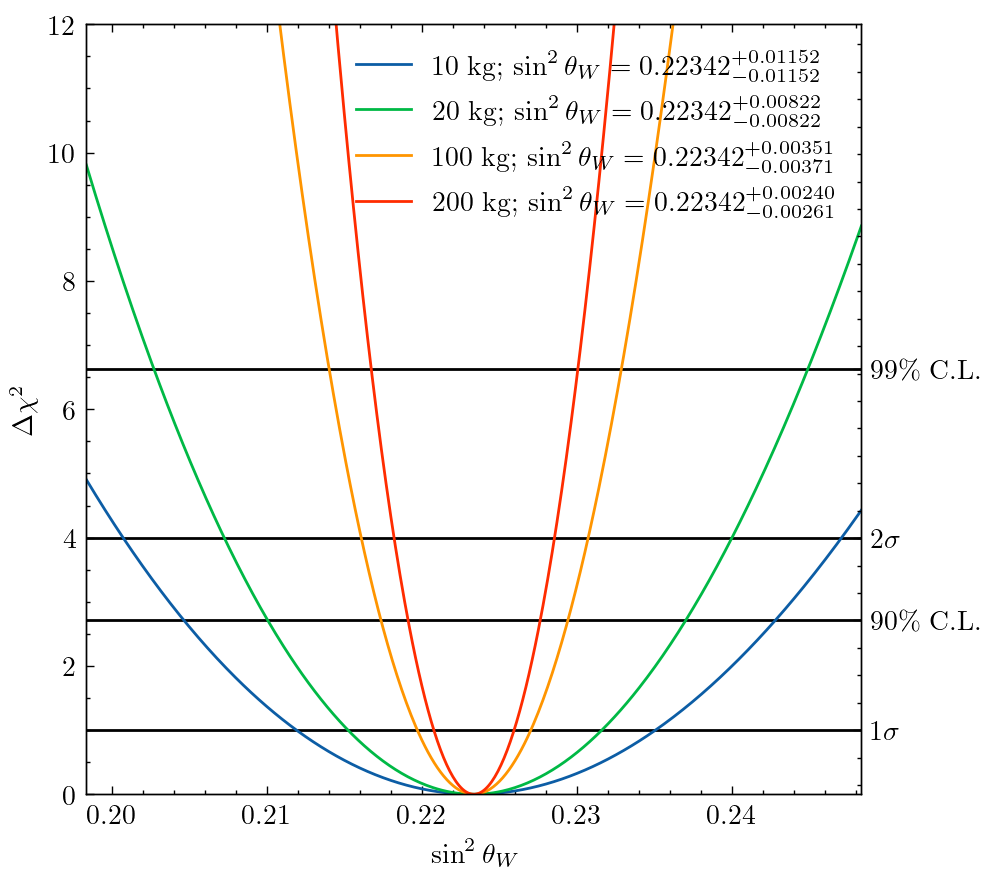
\includegraphics[width=0.5\textwidth]{figures/Figure_sin_200.png}
% \caption{$\Delta\chi^2$ curves for the parameter $\sin^2\theta_W$, experimental arrangement with 200-day exposure, including quenching factor.}
% \label{fig:chi2_sin2thetaW_200d_QF}
% \end{figure}



\subsubsection{Sensitivity to \texorpdfstring{$\langle r_{\nu_e}^2\rangle$}{NCR}}

For an experiment with 100-day exposure, including the Lindhard quenching factor, the values at $1\sigma$ confidence level are given by:
\begin{itemize}
\item $\langle r_{\nu_e}^2\rangle = -8\pm13\times10^{-33}\ \text{cm}^2$, 10 kg detector.
\item $\langle r_{\nu_e}^2\rangle = -8\pm9\times10^{-33}\ \text{cm}^2$, 20 kg detector.
\item $\langle r_{\nu_e}^2\rangle = -8\pm4\times10^{-33}\ \text{cm}^2$, 100 kg detector.
\item $\langle r_{\nu_e}^2\rangle = -8\pm3\times10^{-33}\ \text{cm}^2$, 200 kg detector.
\end{itemize}

% \begin{figure}[H]
% \centering
% 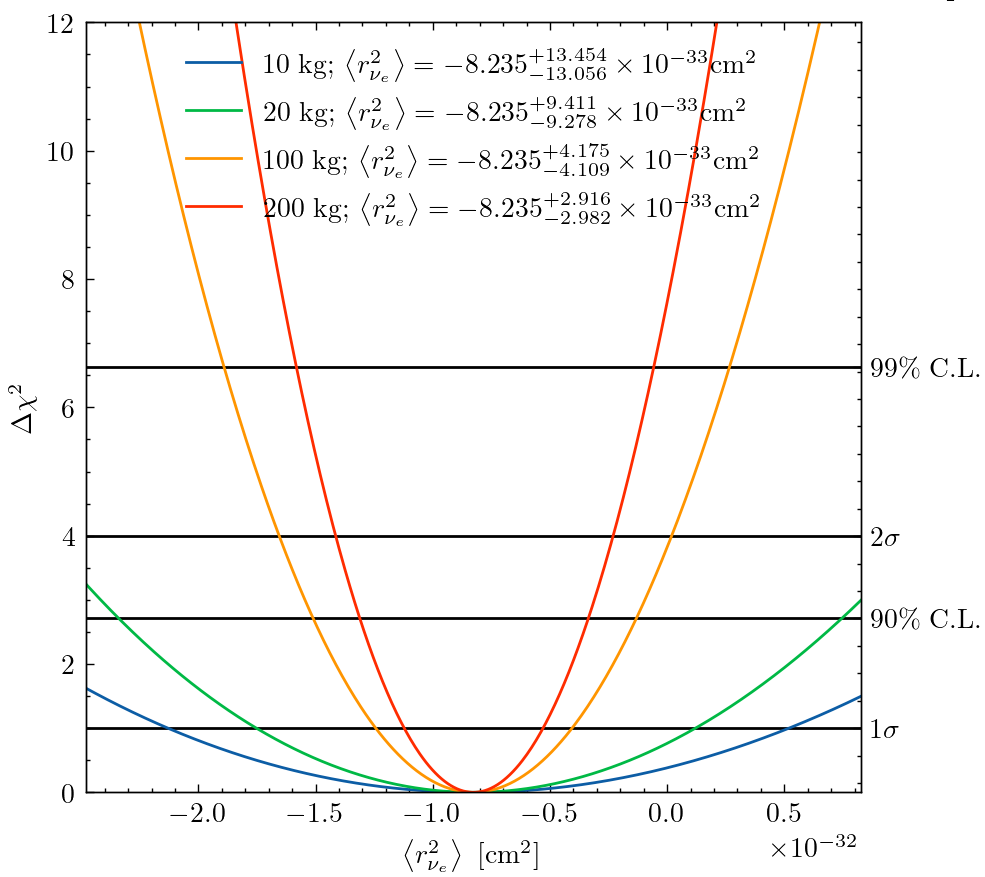
\includegraphics[width=0.5\textwidth]{figures/Figure_phi_100.png}
% \caption{$\Delta\chi^2$ curves for the parameter $\langle r_{\nu_e}^2\rangle$, experimental arrangement with 100-day exposure, including quenching factor.}
% \label{fig:chi2_NCR_100d_QF}
% \end{figure}

For an experiment with 200-day exposure, including the Lindhard quenching factor, the values at $1\sigma$ confidence level are given by:
\begin{itemize}
\item $\langle r_{\nu_e}^2\rangle = -8\pm9\times10^{-33}\ \text{cm}^2$, 10 kg detector.
\item $\langle r_{\nu_e}^2\rangle = -8\pm6\times10^{-33}\ \text{cm}^2$, 20 kg detector.
\item $\langle r_{\nu_e}^2\rangle = -8\pm3\times10^{-33}\ \text{cm}^2$, 100 kg detector.
\item $\langle r_{\nu_e}^2\rangle = -8\pm2\times10^{-33}\ \text{cm}^2$, 200 kg detector.
\end{itemize}


% \begin{figure}[H]
% \centering
% 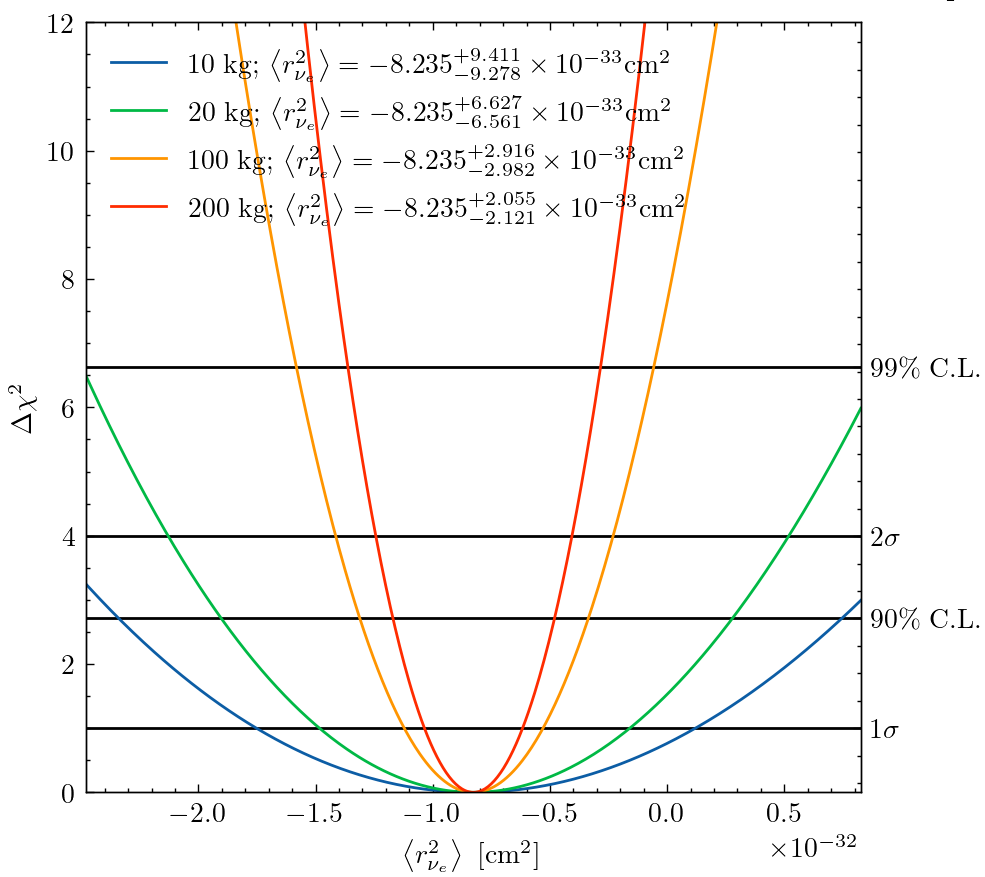
\includegraphics[width=0.5\textwidth]{figures/Figure_phi_200.png}
% \caption{$\Delta\chi^2$ curves for the parameter $\langle r_{\nu_e}^2\rangle$, experimental arrangement with 200-day exposure, including quenching factor.}
% \label{fig:chi2_NCR_200d_QF}
% \end{figure}


\begin{figure}[H]
\centering
\subfigure[100-day exposure.]{
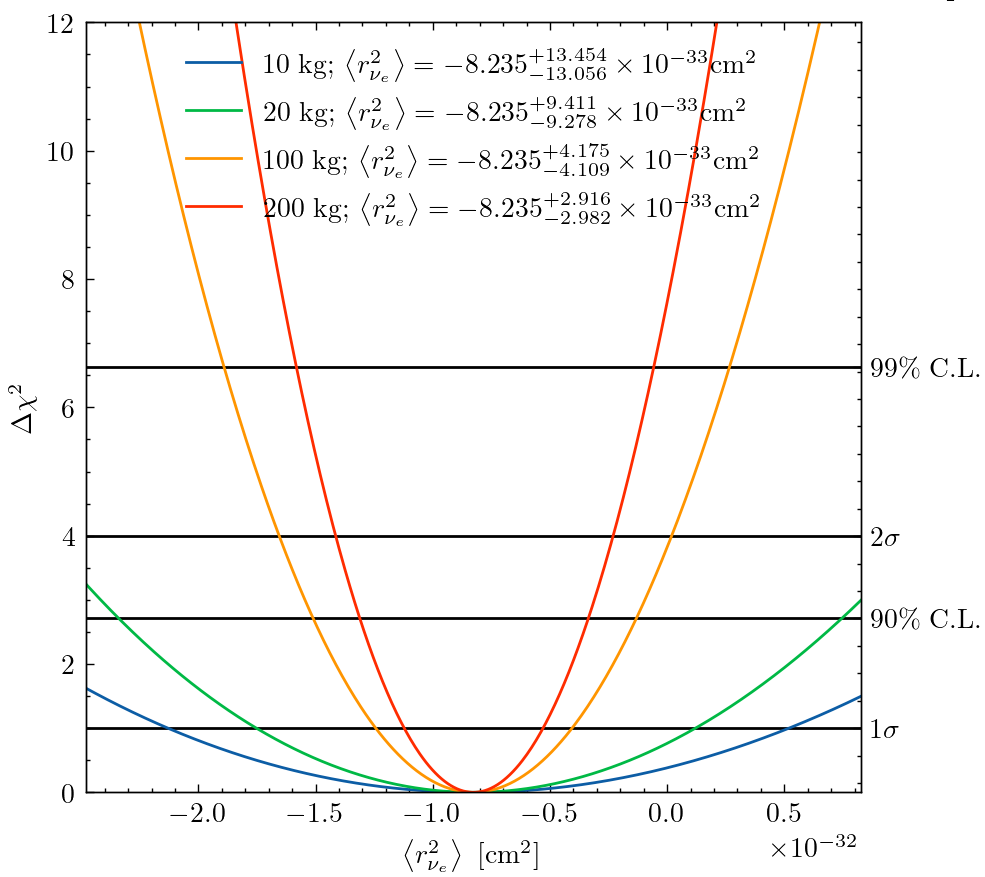
\includegraphics[width=0.48\textwidth]{figures/Figure_phi_100.png}
\label{fig:chi2_sin2thetaW_100d}}
\subfigure[200-day exposure.]{
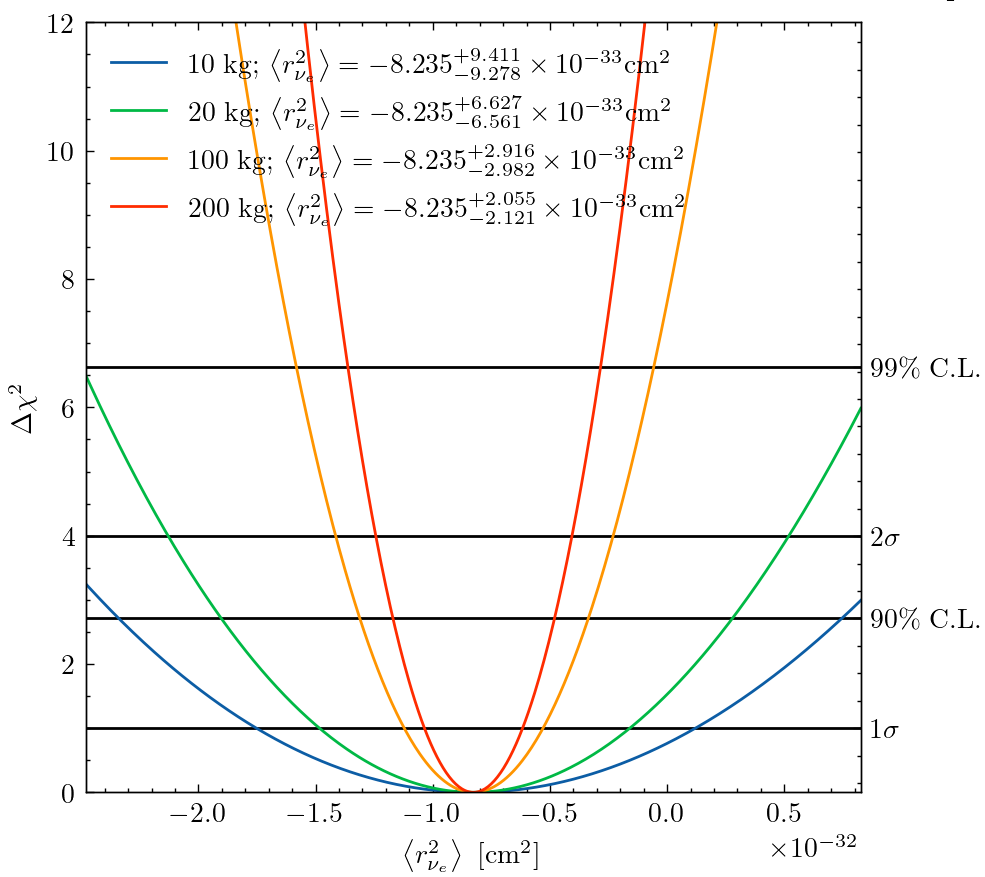
\includegraphics[width=0.48\textwidth]{figures/Figure_phi_200.png}
\label{fig:chi2_sin2thetaW_200d}}
\caption{$\Delta\chi^2$ curves for the parameter $\langle r^2_{\nu_e} \rangle$, with Lindhard QF influence.}
\label{fig:chi2_sin2thetaW_noQF}
\end{figure}
